%!TEX program = xelatex
\documentclass[11pt,class=book]{standalone}
%\usepackage[utf8]{inputenc}
\usepackage[french]{babel}
\usepackage[french]{translator}
\usepackage[T1]{fontenc}
\usepackage{fontspec}
\usepackage[table,svgnames]{xcolor}

\usepackage{pgf}
\usepackage{tikz}

\usetikzlibrary{shapes}
\usetikzlibrary{arrows.meta}
\usetikzlibrary{calc}
\usetikzlibrary{matrix}


\begin{document}
	\begin{tikzpicture}[x=1pt,y=1pt,>=Latex]
		\node[
			anchor=south west,
			inner sep=0
		] (image) at (0,0)
		{\setlength{\fboxsep}{0pt}\fbox{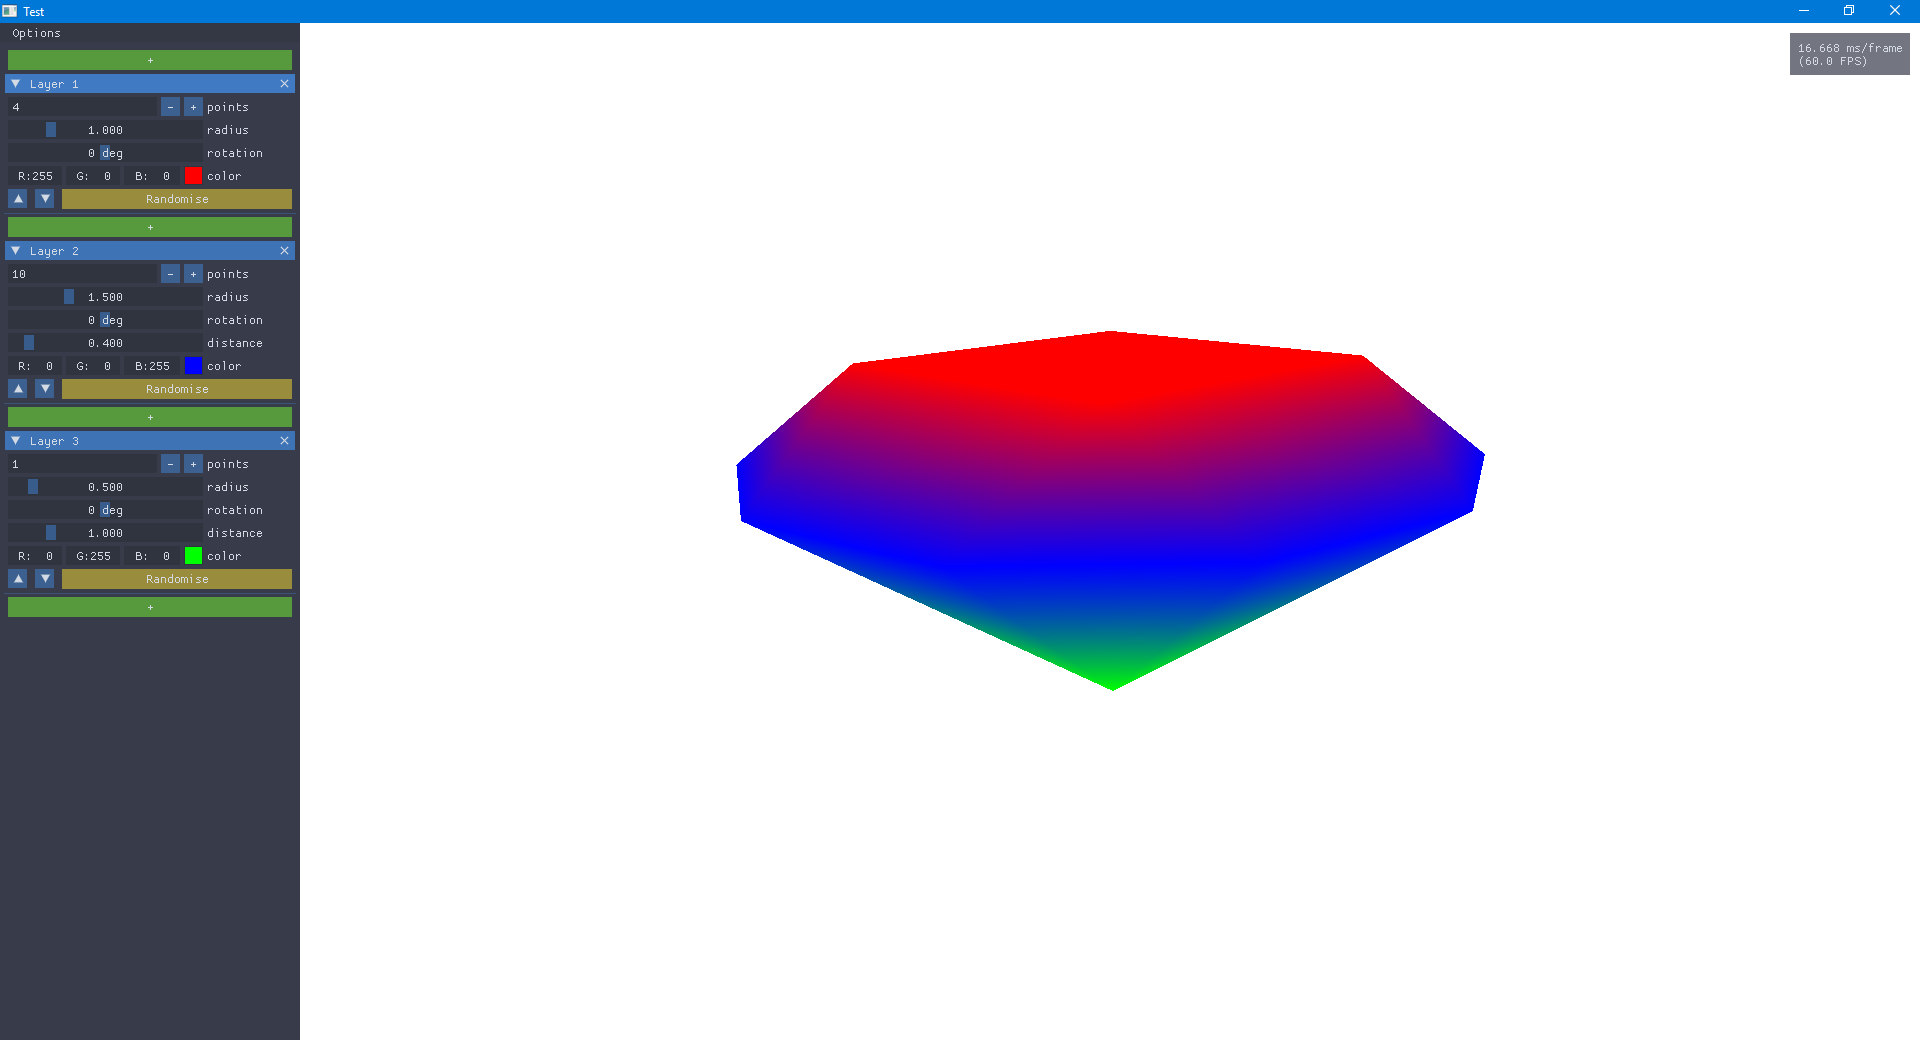
\includegraphics[width=0.9\textwidth]{capture}}};

		\begin{scope}[x={(image.south east)},y={(image.north west)}]
			%\draw[help lines,xstep=.1,ystep=.1] (0,0) grid (1,1);
			%\foreach \x in {0,1,...,9} { \node [anchor=north] at (\x/10,0) {\tiny 0.\x}; }
			%\foreach \y in {0,1,...,9} { \node [anchor=east] at (0,\y/10) {\tiny 0.\y}; }
			\draw[->,thick,red,text=black] (0.5,0.99) node[circle,minimum size=5,inner sep=0,fill=red] {} -- ++(0,0.1) node[above] {GLFW};
			\draw[->,thick,red,text=black] (0.05,0.3) node[circle,minimum size=5,inner sep=0,fill=red] {} -- ++(-0.1,0) node[left] {ImGUI};
			\draw[->,thick,red,text=black] (0.95,0.7) node[circle,minimum size=5,inner sep=0,fill=red] {} -- ++(0.1,0) node[right] {OpenGL};
		\end{scope}
	\end{tikzpicture}
\end{document}
